\documentclass[11pt]{article}
\usepackage[margin=0.85in]{geometry}
\usepackage{graphicx}
\usepackage{amsmath,amssymb}
\title{Native Replay Record: Prime-Field Cover Sections}
\author{Run enge-primefield-cover-20261024-native-2315Z}
\date{24 October 2026, 23:15 UTC}
\begin{document}
\maketitle
\noindent\textbf{Host and isolation.}
Intel Xeon 6975P-C, x86-64, 32 logical CPUs, shared EC2 host.
No CPU pinning or isolated timing claim. One exhaustive census was
requested and completed for each of $(d,s)=(2,0),(3,0),(5,0),(7,0),(2,6)$.
The input is the public $E/\mathbb F_{101}:y^2=x^3+x+46$ with
$G=(2,37)$ and $Q=(64,19)$. The code uses deterministic loops and rho salts.
The command and raw JSON record are named in the adjacent \texttt{REPORT.md}.

\begin{center}
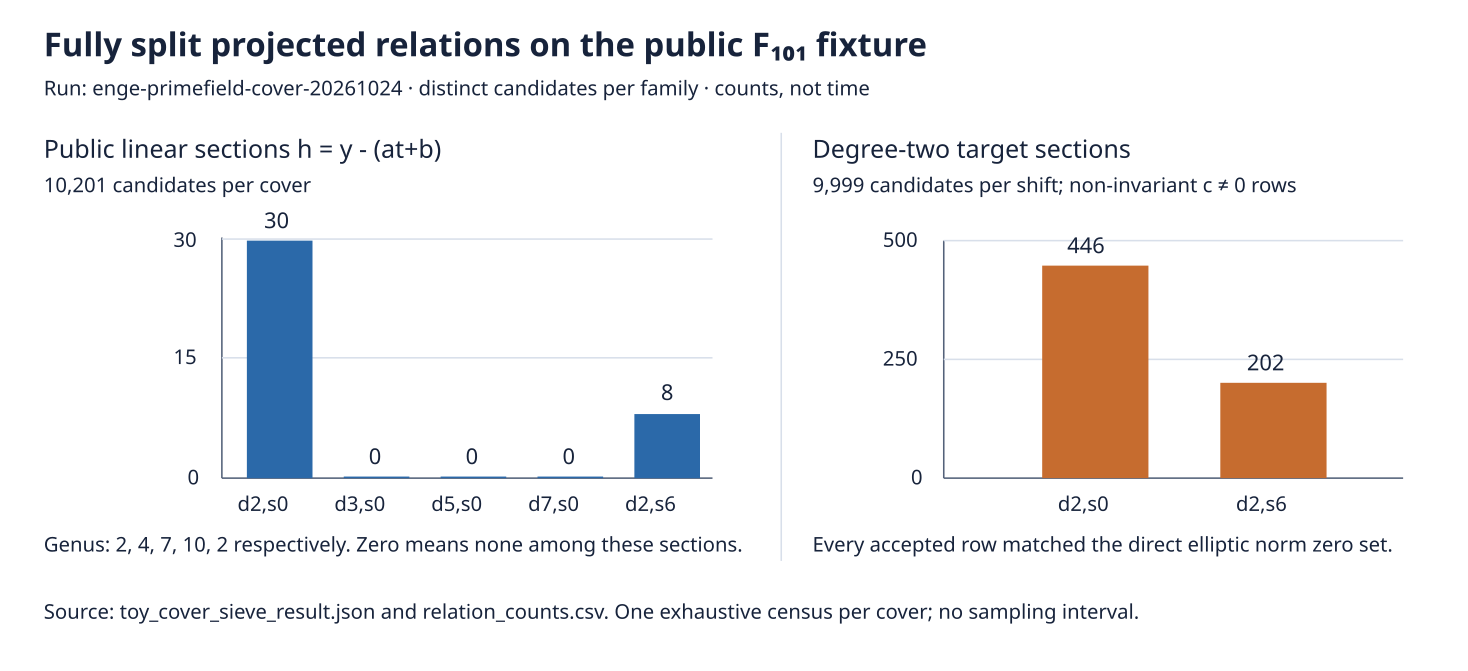
\includegraphics[width=0.98\linewidth]{../../relation_counts.png}
\end{center}

\noindent\textbf{Observed counts.}
The five public-section split counts were $30,0,0,0,8$ of $10{,}201$
candidates per cover. The two degree-two target-section native counts were
$446$ and $202$ of $9{,}999$ candidates per shift. Every one of the $202$
accepted $(2,6)$ rows matched the direct elliptic norm zero set.
Target-only streaming found the verified scalar $37$ after $1{,}070$
candidates, $108{,}070$ cover-point tests, and $22$ accepted rows.
The signed matrix rank was $21$ on $22$ columns. The deterministic rho
control required $72$ elliptic group operations through collision.

\noindent\textbf{Scope.}
These are complete deterministic counts for the stated families and one
run per cover, with no sampling interval. The units of the cover and rho
counts differ; wall time, memory, setup and shift selection were not
measured. No speed ratio is supported. The root \texttt{REPORT.pdf}
contains the algebra and interpretation.
\end{document}
